\documentclass[10 pt]{beamer}
\usetheme{Madrid}
\usepackage[utf8]{inputenc}
\usepackage{xspace}
\usepackage{graphicx,graphics} 
\usepackage{color}
\usepackage{amsmath}
\usepackage{amsfonts}
\usepackage{amssymb}
\usepackage{amsthm}
\usepackage{algorithm}
\usepackage{algorithmic}
\usepackage{longtable}
\usepackage{complexity}
\usepackage{tkz-graph}
\usepackage{float}
\usepackage{multicol}
\usepackage{setspace}
\usepackage[absolute,overlay]{textpos}
\graphicspath{{fig/}}

\tikzset{
  LabelStyle/.style = { rectangle, rounded corners, draw,
                       font = \bfseries },
  EdgeStyle/.append style = {-} }
\title{Deterministic Scheduling of Periodic Messages for Cloud RAN}

\author{{\bf Maël~Guiraud}}


\institute[Nokia Bell Labs, DAVID-UVSQ] 
{
  DAVID, Universit\'e de Versailles Saint Quentin -
  Nokia Bell Labs France \\
}

\subject{Theoretical Computer Science}

\begin{document}


\begin{frame}

  \titlepage
  \centering
  
\includegraphics [width=15mm]{logod.png} \hspace{1cm} 
\includegraphics [width=20mm]{logon.png} \hspace{1cm} 
\includegraphics [width=20mm]{logo.png} \\
\end{frame}




\begin{section}{Introduction}

\begin{frame}{Context}
  \centering
    A Base Transceiver Station
  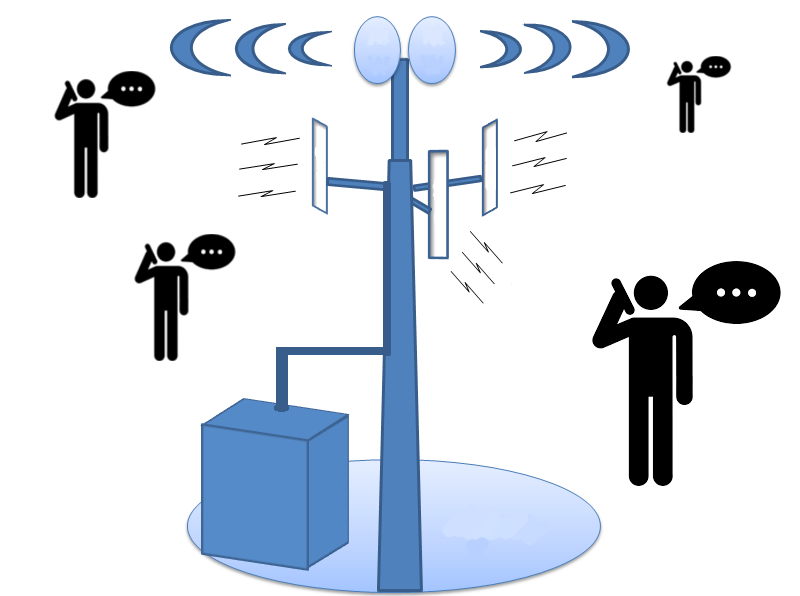
\includegraphics[scale=0.3]{btsppl.png}

\end{frame}


\begin{frame}{Context}
  \centering
  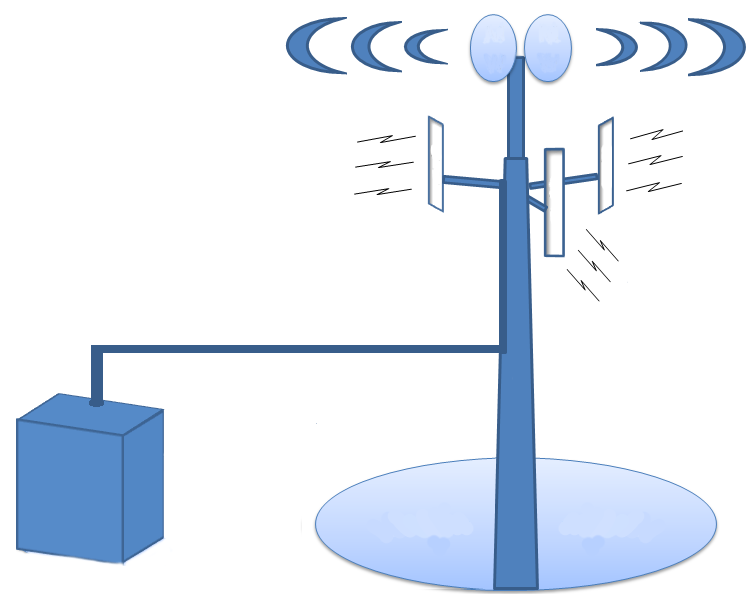
\includegraphics[scale=0.2]{cloudbts.png}\\
  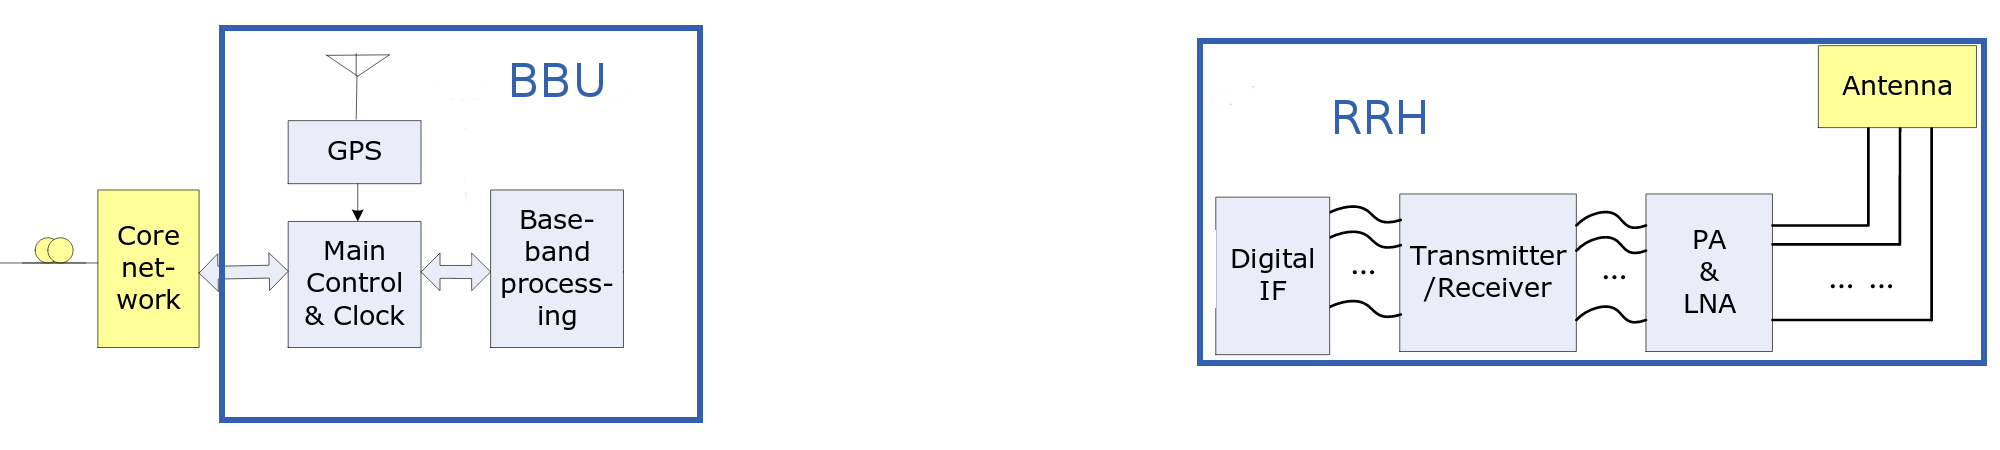
\includegraphics[scale=0.175]{BBURRH.png}
\end{frame}



\begin{frame}{Context}
  \centering
  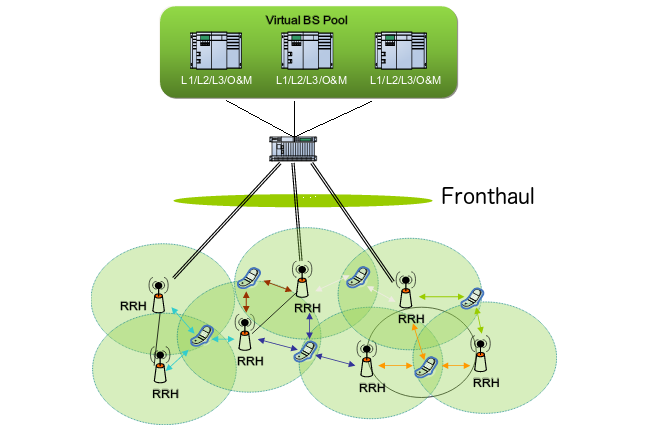
\includegraphics[scale=0.5]{CRAN}\\
  
\end{frame}

\begin{frame}{Problematic}
  \centering
  
  
 \begin{multicols}{2}
Constraints in Fronthaul network :
\vspace{1cm}
\begin{itemize}
\item Highly loaded
\item Periodic traffic
\item \textcolor{red}{Latency must be guaranteed}
\end{itemize}
\vspace{0.5cm}
Current approaches: \begin{itemize}
\vspace{1cm}
\item PtP connections $\rightarrow$ Too expensive
\item Statistical multiplexing $\rightarrow$ No latency guarantees  
\end{itemize}
\end{multicols}

\end{frame}

\end{section}

\begin{section}{Model, Problem}

\begin{subsection}{Network Modeling}

\begin{frame}{Model}

\centering
\scalebox{0.4}{

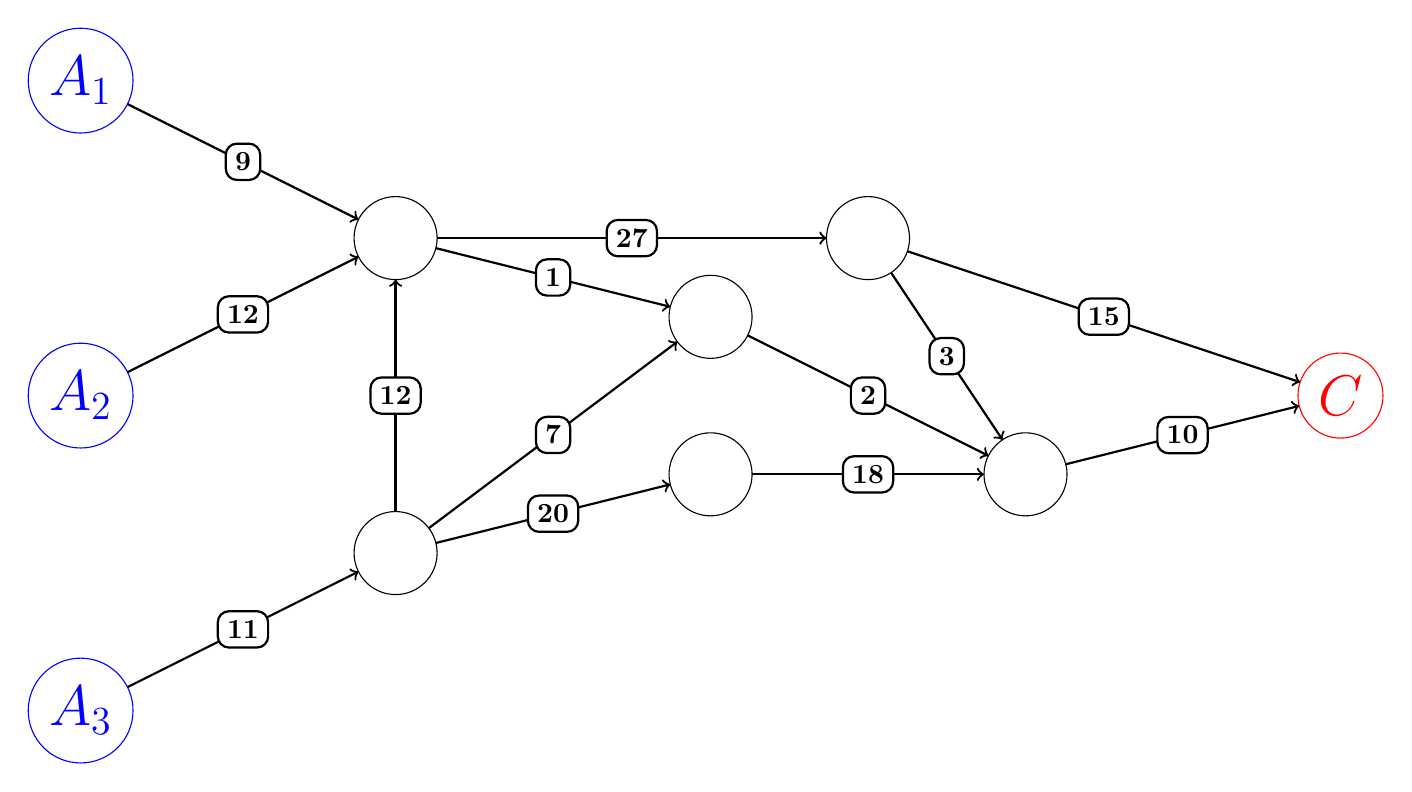
\begin{tikzpicture}
  \SetGraphUnit{5}
    \tikzset{
  EdgeStyle/.append style = {->} }
   \tikzstyle{VertexStyle}=[shape = circle, draw, minimum size = 30pt]
   \renewcommand{\VertexLightFillColor}{orange}
  \Vertex[x=0,y=0, L = {\huge $A_3$},style={blue}]{a3};
  \Vertex[x=0,y=4, L = {\huge $A_2$},style={blue}]{a2}
  \Vertex[x=0,y=8, L = {\huge $A_1$},style={blue}]{a1}


  \Vertex[x=16,y=4, L = {\huge $C$},style={red}]{c}
  
 \SetVertexNoLabel
  \Vertex[x=4,y=2]{n1}
  \Vertex[x=4,y=6]{n2}  
  \Vertex[x=12,y=3]{n4}
  \Vertex[x=8,y=3]{n6}
  \Vertex[x=8,y=5]{n7}
  \Vertex[x=10,y=6]{n8}



  \Edge[label = 12](n1)(n2)
  \Edge[label = 3](n8)(n4)
  \Edge[label = 15](n8)(c)
  \Edge[label = 27](n2)(n8)
  \Edge[label = 7](n1)(n7)
  \Edge[label = 9](a1)(n2)   
  \Edge[label = 2](n7)(n4)
  \Edge[label = 11](a3)(n1)
  \Edge[label = 20](n1)(n6)
  \Edge[label = 18](n6)(n4)
  \Edge[label = 12](a2)(n2)
  \Edge[label = 10](n4)(c)
  \Edge[label = 1](n2)(n7)

 
\end{tikzpicture}
}
\vspace{1cm}
\begin{itemize}
\item Network : Weighted Directed Graph
\item RRH / BBU $\rightarrow$ set of vertices \textcolor{blue}{A (Antennas)} and \textcolor{red}{C (Computation)}
\item  Physical Delay of a link $\rightarrow$ Weight of the arc
\end{itemize}

 \end{frame}
 
 
\begin{frame}{Routed Network}

\begin{center}
\scalebox{0.4}{

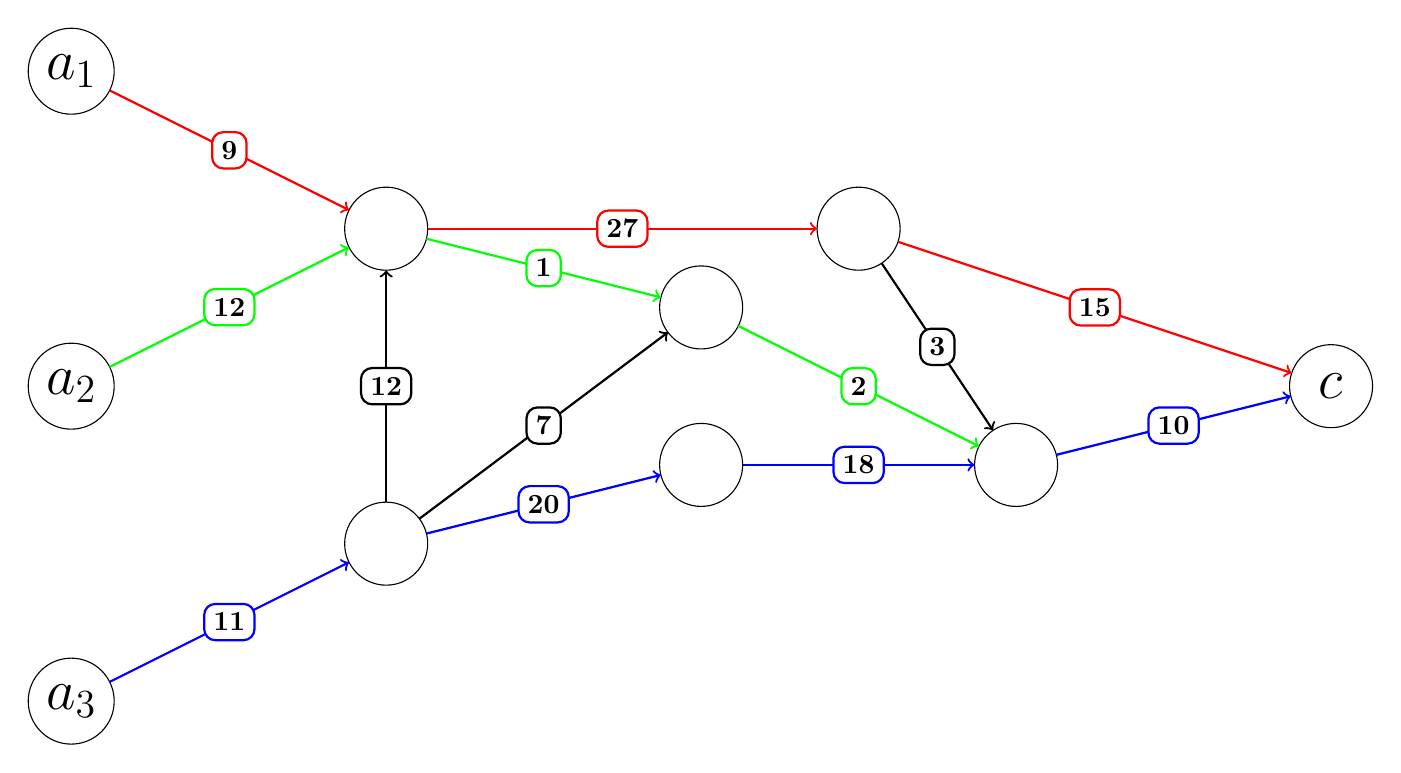
\begin{tikzpicture}
  \SetGraphUnit{5}
    \tikzset{
  EdgeStyle/.append style = {->} }
   \tikzstyle{VertexStyle}=[shape = circle, draw, minimum size = 30pt]
   \renewcommand{\VertexLightFillColor}{orange}
  \Vertex[x=0,y=0, L = {\huge $a_3$}]{a3};
  \Vertex[x=0,y=4, L = {\huge $a_2$}]{a2}
  \Vertex[x=0,y=8, L = {\huge $a_1$}]{a1}


  \Vertex[x=16,y=4, L = {\huge $c$}]{c}
  
 \SetVertexNoLabel
  \Vertex[x=4,y=2]{n1}
  \Vertex[x=4,y=6]{n2}  
  \Vertex[x=12,y=3]{n4}
  \Vertex[x=8,y=3]{n6}
  \Vertex[x=8,y=5]{n7}
  \Vertex[x=10,y=6]{n8}



  \Edge[label = 12](n1)(n2)
  \Edge[label = 3](n8)(n4)

  \Edge[label = 7](n1)(n7)

    
      \tikzset{
  EdgeStyle/.append style = {->,red} }
    \Edge[label = 9](a1)(n2)   
    \Edge[label = 15](n8)(c)
  \Edge[label = 27](n2)(n8)
  
      \tikzset{
  EdgeStyle/.append style = {->,blue} }
  \Edge[label = 11](a3)(n1)
  \Edge[label = 20](n1)(n6)
  \Edge[label = 18](n6)(n4)
  \Edge[label = 10](n4)(c) 
  
  
  
        \tikzset{
  EdgeStyle/.append style = {->,green} }
  
  
  \Edge[label = 2](n7)(n4)

  \Edge[label = 12](a2)(n2)

  \Edge[label = 1](n2)(n7)
\end{tikzpicture}
}
\vspace{1cm}
\end{center}
There is a route going from each RRH to the BBU.\\

A {\bf routed network} : set of routes.
 \end{frame}

 
 \begin{frame}{The communication process}
Two parameters
\begin{itemize}
\item The period $P$
\item The size of a message $\tau$
\end{itemize}
\vspace{0.5cm}
The time is discretized and on each route of the network, every $P$ units of time, a message of size $\tau$ is emitted.

\vspace{0.5cm}
\begin{center}
  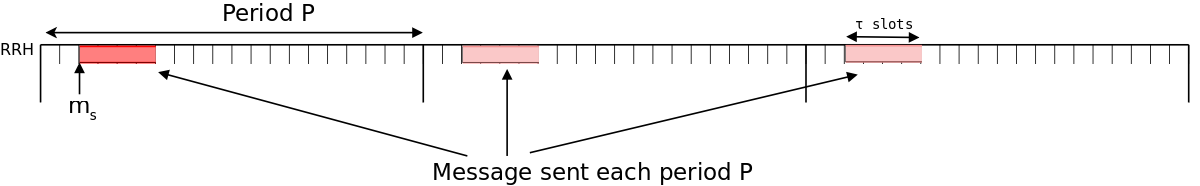
\includegraphics [width=11.5cm]{rrh} 
  \end{center}
 \vspace{0.5cm}
   
   The process is \textcolor{red}{periodic} : the message is emitted in each period at the same time, called \textcolor{blue}{offset}.
   
\end{frame}


 \begin{frame}{Collisions}

\begin{center}
\scalebox{0.4}{

\begin{tikzpicture}
  \SetGraphUnit{5}
    \tikzset{
  EdgeStyle/.append style = {->} }
   \tikzstyle{VertexStyle}=[shape = circle, draw, minimum size = 30pt]
   \renewcommand{\VertexLightFillColor}{orange}
  \Vertex[x=0,y=0, L = {\huge $a_3$}]{a3};
  \Vertex[x=0,y=4, L = {\huge $a_2$}]{a2}
  \Vertex[x=0,y=8, L = {\huge $a_1$}]{a1}


  \Vertex[x=16,y=4, L = {\huge $c$}]{c}
  
 \SetVertexNoLabel
  \Vertex[x=4,y=2]{n1}
  \Vertex[x=4,y=6]{n2}  
  \Vertex[x=12,y=3]{n4}
  \Vertex[x=8,y=3]{n6}
  \Vertex[x=8,y=5]{n7}
  \Vertex[x=10,y=6]{n8}



  \Edge(n1)(n2)
  \Edge(n8)(n4)
  \Edge(n8)(c)
  \Edge(n2)(n8)
  \Edge(n7)(n4)
  \Edge(n1)(n6)
  \Edge(n6)(n4)
  \Edge(a2)(n2)
  \Edge(n4)(c)

    
  \tikzset{
  EdgeStyle/.append style = {blue} }
  \Edge[label = 5](a1)(n2)   
   \Edge[label = 3](n2)(n7)
  
    \tikzset{
  EdgeStyle/.append style = {red} }
    \Edge[label = 2](a3)(n1)
      \Edge[label = 6](n1)(n7)
      
       \node (0) at (9,4){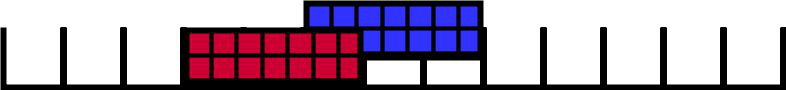
\includegraphics[scale=0.2]{col1.png}};


\end{tikzpicture}
}
\end{center}
\vspace{1cm}
\centering
There is a \textcolor{blue}{collision} between two routes when their messages go through the first vertex of a common arc at the same time.
\vspace{0.5cm}

 \textcolor{red}{Periodicity must be taken into consideration} 
\end{frame}

 \begin{frame}{Assignment }

\begin{center}
\scalebox{0.4}{

\begin{tikzpicture}
  \SetGraphUnit{5}
    \tikzset{
  EdgeStyle/.append style = {->} }
   \tikzstyle{VertexStyle}=[shape = circle, draw, minimum size = 30pt]
   \renewcommand{\VertexLightFillColor}{orange}
  \Vertex[x=0,y=0, L = {\huge $a_3$}]{a3};
  \Vertex[x=0,y=4, L = {\huge $a_2$}]{a2}
  \Vertex[x=0,y=8, L = {\huge $a_1$}]{a1}


  \Vertex[x=16,y=4, L = {\huge $c$}]{c}
  
 \SetVertexNoLabel
  \Vertex[x=4,y=2]{n1}
  \Vertex[x=4,y=6]{n2}  
  \Vertex[x=12,y=3]{n4}
  \Vertex[x=8,y=3]{n6}
  \Vertex[x=8,y=5]{n7}
  \Vertex[x=10,y=6]{n8}



  \Edge(n1)(n2)
  \Edge(n8)(n4)
  \Edge(n8)(c)
  \Edge(n2)(n8)
  \Edge(n7)(n4)
  \Edge(n1)(n6)
  \Edge(n6)(n4)
  \Edge(a2)(n2)
  \Edge(n4)(c)

    
  \tikzset{
  EdgeStyle/.append style = {blue} }
  \Edge[label = 5](a1)(n2)   
   \Edge[label = 3](n2)(n7)
  
    \tikzset{
  EdgeStyle/.append style = {red} }
    \Edge[label = 2](a3)(n1)
      \Edge[label = 6](n1)(n7)
      
       \node (0) at (9,4){
\includegraphics[scale=0.2]{col2.png}};


\end{tikzpicture}
}
\end{center}
\vspace{1cm}
\centering
Choosing the offset such that there are no collisions.
\vspace{0.5cm}

An \textcolor{blue}{assignment} is a choice of offsets for each route without collisions.
\end{frame}
\end{subsection}



\begin{subsection}{Problem PALL}
\begin{frame}{Full process}
In each BBU, one can choose the \textcolor{blue}{waiting time} before sending back the answer.\\

\begin{center}
  \includegraphics[scale=0.7]{BBU}\\
 \end{center} 
Two different problems:
 \begin{multicols}{2}
PALL :
\begin{itemize}
\item The RRH send their message at different dates in the period.
\item Local latency constraint.
\item Minimizing the process time on the longest route.
\end{itemize}
\vspace{0.5cm}
SPALL
\begin{itemize}
\item The RRH send their message at the same date (Synchronized).
\item Global time constraint.
\item Minimizing the time between the emission of the first message and the reception of the last message.
\end{itemize}
\end{multicols}
\end {frame}
\end{subsection}


\end{section}

\begin{section}{Results on a common topology}

\begin{subsection}{A star routed Network}
\begin{frame}{Different topologies}

The  {\bf conflict depth} of a route is defined as the number of arcs shared with other routes.
  \centering
   \begin{multicols}{2}


\scalebox{0.25}{
\begin{tikzpicture}
    \SetGraphUnit{5}
  \tikzstyle{VertexStyle}=[shape = circle, draw, minimum size = 50pt]
  \Vertex[x=0,y=0]{a3}
  \Vertex[x=0,y=4]{a2}
  \Vertex[x=0,y=8]{a1}
  
  \Vertex[x=16,y=0]{c3}
  \Vertex[x=16,y=4]{c2}
  \Vertex[x=16,y=8]{c1}
  
  \SetVertexNoLabel
  \Vertex[x=4,y=4]{SL}
  \Vertex[x=12,y=4]{SS}  
  \tikzset{
  EdgeStyle/.append style = {<-,green} }
  \Edge(c1)(SS)
  \Edge(SL)(a1)
  
  \tikzset{
  EdgeStyle/.append style = {blue} }
  \Edge(c2)(SS)
  \Edge(SL)(a2)
  
  \tikzset{
  EdgeStyle/.append style = {red} }
  \Edge(c3)(SS)
  \Edge(SL)(a3)
  
  \tikzset{
  EdgeStyle/.append style = {black} }
  \Edge(SS)(SL)
  


\end{tikzpicture}
}

 \vspace{1cm}
\centering
 Conflict depth one.
 

 

 
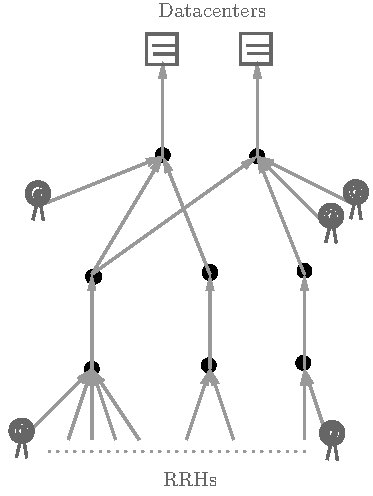
\includegraphics[scale=0.5]{extendendgraphgrey}\\
 \centering

 Conflict depth two.

\end{multicols}
\end{frame}

\begin{frame}{NP-Hardness}
   \begin{multicols}{2}
   PALL:
   \begin{itemize}
   \item Hard on conflict depth $2$ : reduction of a k-coloring problem
   \item Hard on conflict depth $1$ if the shared arc is bidirectional.
   \end{itemize}
   
   SPALL:
   \begin{itemize}
   \item Hard on conflict depth $1$ : reduction of a two processor scheduling problem.
   \end{itemize}
   \end{multicols}

\end{frame}
\end{subsection}

\begin{subsection}{Solving PALL}
\begin{frame}{Solving PALL on conflict depth $1$ : a two stages approach}

{\bf First step}. We fix the offsets of the forward routes according to several heuristics.
\vspace{0.5cm}


{\bf Second step}. Algorithms to schedule the backward routes.
\vspace{0.5cm}
\begin{itemize}
	
	 \item A greedy algorithm (GD)
	 \item Scheduling algorithm adapted for periodicity (PMLS)
	 \item FPT algorithm (FPT-PMLS)
	\end{itemize}


\end{frame}
\end{subsection}

\begin{subsection}{Results}

  \begin{frame}{Performances of the algorithms}
\centering

  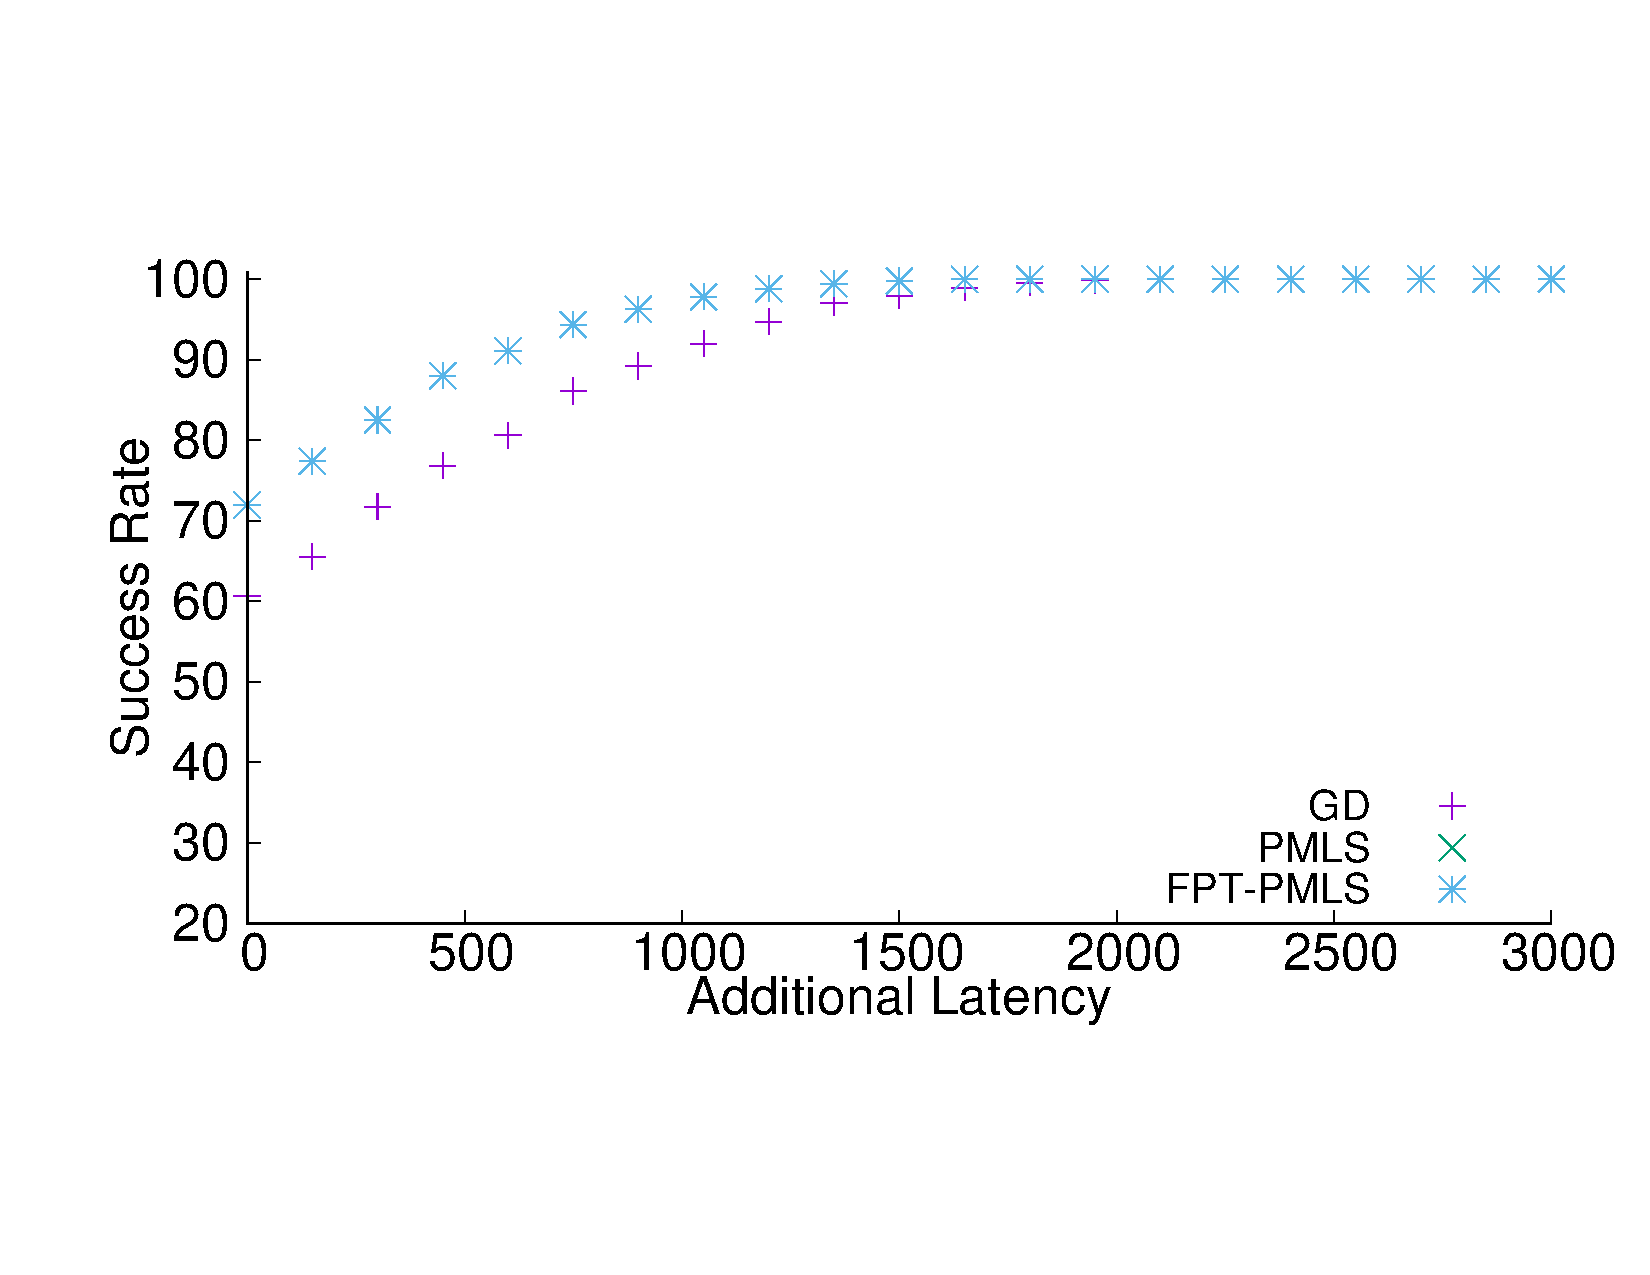
\includegraphics[scale=0.4]{retour_21000.pdf}\\
  \end{frame}
  
    \begin{frame}{Deterministic vs Stochastic}
\centering
\vspace{-2cm}
  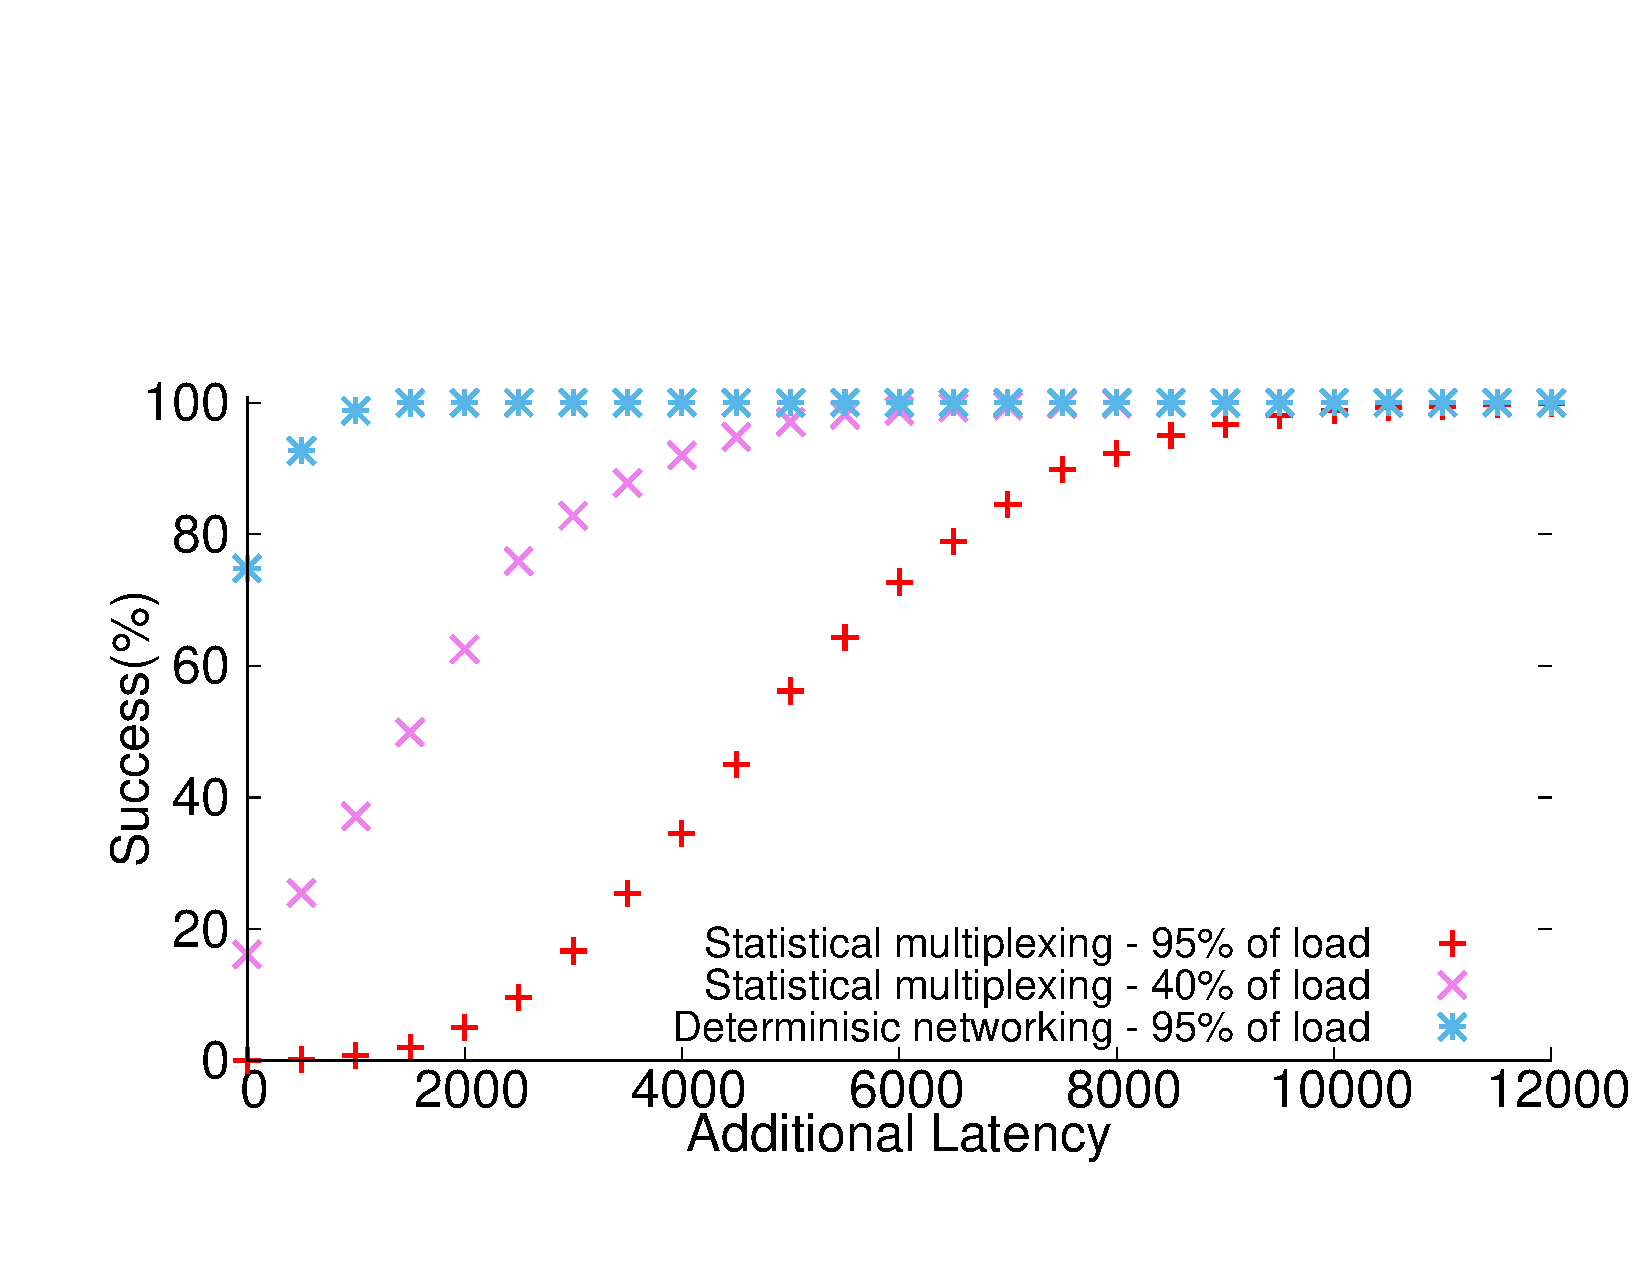
\includegraphics[scale=0.4]{stochastic.pdf}\\
  \end{frame}
  
  
  \begin{frame}{SPALL on conflict depth $1$}
  FPT algorithm to solve SPALL:
  \begin{itemize}
  \item Try all the orders in the way forward
  \item Use FPT-PMLS in the way backward
  \end{itemize}
  \end{frame}
\end{subsection}


\end{section}



\begin{section}{Optical ring}
\begin{frame}{Optical ring}
\centering
\vspace{1cm}
  \includegraphics[scale=0.8]{interface}\\
\end{frame}

\begin{frame}{Results}
\centering
\vspace{1cm}
  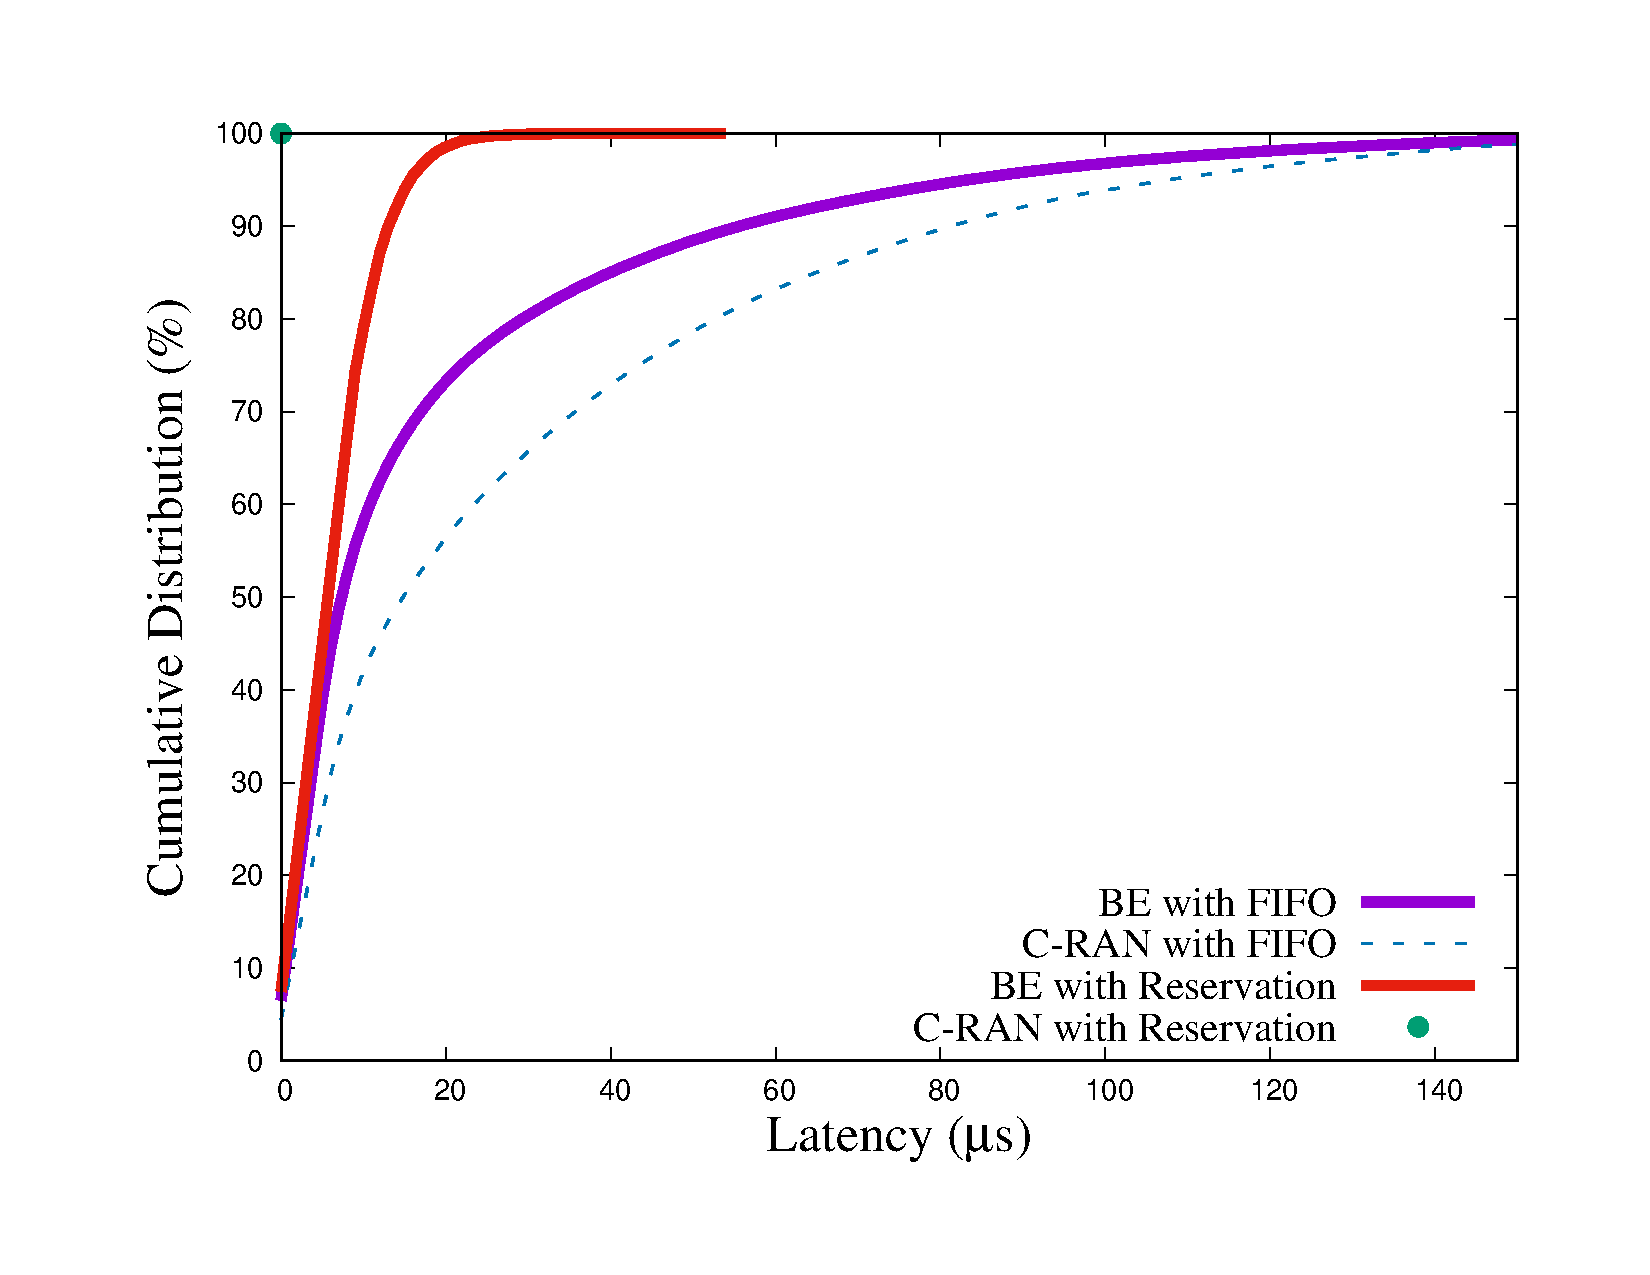
\includegraphics[scale=0.3]{optim}\\

\end{frame}
\end{section}



\begin{section}{Conculsion}
\begin{frame}{Next steps}
\begin{itemize}
\item Solutions for SPALL and SPALL on conflict depth $2$
\vspace{1cm}
\item ...?

\end{itemize}
\vspace{0.5cm}



\end{frame}

\begin{frame}
Thank you for your attention.

\end{frame}
\end{section}

\end{document}
